%Code by GVV Sharma
%December 16, 2019
%released under GNU GPL
%Drawing a right angled triangle: standalone document

\documentclass{article}
\usepackage{rotating}
\usepackage{tikz}
\usepackage{tkz-euclide} % loads  TikZ and tkz-base
%\usetkzobj{all}
\usetikzlibrary{calc,math}

\begin{document}
%\begin{figure}[!ht]
\begin{sidewaysfigure}[!ht]
	\begin{center}
                \resizebox{0.25\columnwidth}{!}{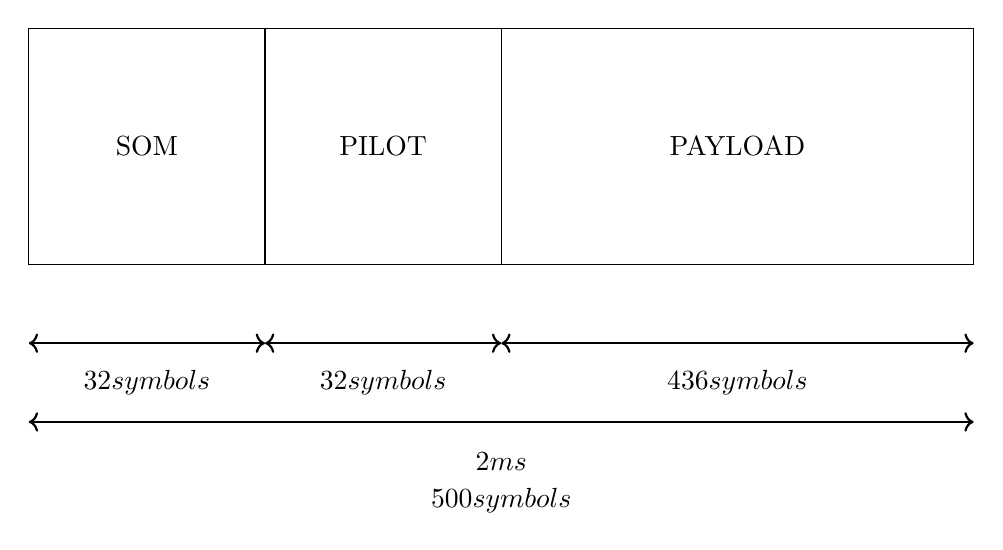
\begin{tikzpicture}


\draw (0,0) -- (12,0);
\draw (0,0) -- (0,-3) -- (12,-3) -- (12,0);
\draw (3,0) -- (3,-3);
\draw (6,0) -- (6,-3);


\node [align=center] at (1.5,-1.5) {SOM};
\node [align=center] at (4.5,-1.5) {PILOT};
\node [align=center] at (9,-1.5) {PAYLOAD};

\draw[<->,thick] (0,-4)--(3,-4) node[align = center] at (1.5,-4.5) {$32 symbols$};
\draw[<->,thick] (3,-4)--(6,-4) node[align = center] at (4.5,-4.5) {$32 symbols$};
\draw[<->,thick] (6,-4)--(12,-4) node[align = center] at (9,-4.5) {$436 symbols$};
\draw[<->,thick] (0,-5)--(12,-5) node[align = center] at (6,-5.5) {$2ms$};

\node [align=center] at (6,-6) {$500 symbols$};



\end{tikzpicture}
}
% 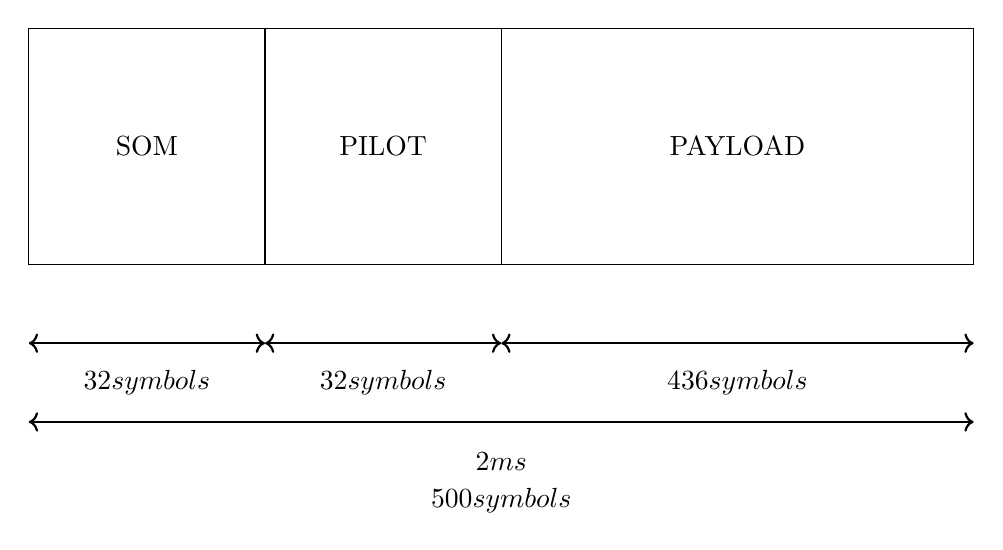
\begin{tikzpicture}


\draw (0,0) -- (12,0);
\draw (0,0) -- (0,-3) -- (12,-3) -- (12,0);
\draw (3,0) -- (3,-3);
\draw (6,0) -- (6,-3);


\node [align=center] at (1.5,-1.5) {SOM};
\node [align=center] at (4.5,-1.5) {PILOT};
\node [align=center] at (9,-1.5) {PAYLOAD};

\draw[<->,thick] (0,-4)--(3,-4) node[align = center] at (1.5,-4.5) {$32 symbols$};
\draw[<->,thick] (3,-4)--(6,-4) node[align = center] at (4.5,-4.5) {$32 symbols$};
\draw[<->,thick] (6,-4)--(12,-4) node[align = center] at (9,-4.5) {$436 symbols$};
\draw[<->,thick] (0,-5)--(12,-5) node[align = center] at (6,-5.5) {$2ms$};

\node [align=center] at (6,-6) {$500 symbols$};



\end{tikzpicture}

%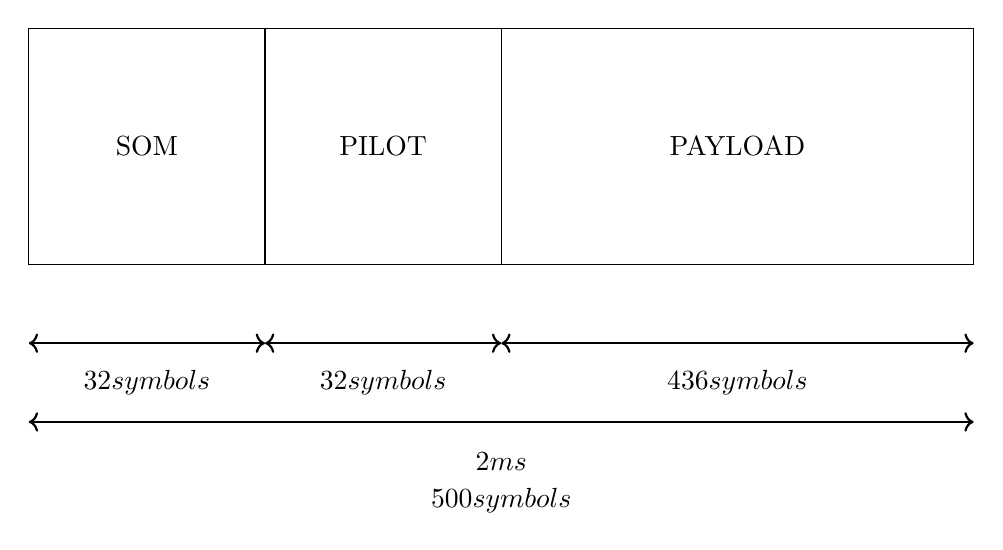
\begin{tikzpicture}


\draw (0,0) -- (12,0);
\draw (0,0) -- (0,-3) -- (12,-3) -- (12,0);
\draw (3,0) -- (3,-3);
\draw (6,0) -- (6,-3);


\node [align=center] at (1.5,-1.5) {SOM};
\node [align=center] at (4.5,-1.5) {PILOT};
\node [align=center] at (9,-1.5) {PAYLOAD};

\draw[<->,thick] (0,-4)--(3,-4) node[align = center] at (1.5,-4.5) {$32 symbols$};
\draw[<->,thick] (3,-4)--(6,-4) node[align = center] at (4.5,-4.5) {$32 symbols$};
\draw[<->,thick] (6,-4)--(12,-4) node[align = center] at (9,-4.5) {$436 symbols$};
\draw[<->,thick] (0,-5)--(12,-5) node[align = center] at (6,-5.5) {$2ms$};

\node [align=center] at (6,-6) {$500 symbols$};



\end{tikzpicture}
		
%\begin{tikzpicture}
%[scale=2,>=stealth,point/.style={draw,circle,fill = black,inner sep=0.5pt},]
%
%%Triangle sides
%\def\a{4}
%\def\c{3}
%
%%Marking coordiantes
%\coordinate [label=above:$A$] (A) at (0,\c);
%\coordinate [label=left:$B$] (B) at (0,0);
%\coordinate [label=right:$C$] (C) at (\a,0);
%
%%Drawing triangle ABC
%\draw (A) -- node[left] {$\textrm{c}$} (B) -- node[below] {$\textrm{a}$} (C) -- node[above,,xshift=2mm] {$\textrm{b}$} (A);
%
%%Drawing and marking angles
%\tkzMarkAngle[fill=orange!40,size=0.5cm,mark=](A,C,B)
%\tkzMarkRightAngle[fill=blue!20,size=.3](A,B,C)
%\tkzLabelAngle[pos=0.65](A,C,B){$\theta$}
%\end{tikzpicture}
	\end{center}
\caption{Right Angled Triangle}
\label{fig:tri_right_angle}	
\end{sidewaysfigure}
%\end{figure}
\end{document}
